\chapter{Implementación}\label{chapter:implementacion}

Es este capítulo se describe la implementación del trabajo, a partir de las decisiones de diseño expuestas en el Capítulo~\ref{chapter:diseno}. Primero, se presenta la estructuración del software en términos de archivos y paquetes ROS. Luego se describe la implementación del sistema LTM: el modelo episódico, el servidor, el sistema de plugins y la API ROS para su utilización. En tercer lugar, se presentan módulos de software implementados para acelerar la implementación y validar el trabajo. Finalmente, se presenta la integración del sistema LTM en el robot Bender.

% ==============================================================================
% ==============================================================================

% ==============================================================================
% ==============================================================================

% ==============================================================================
% ==============================================================================

% ==============================================================================
% ==============================================================================
% ==============================================================================
% ==============================================================================
\section{Estructura del Software}
% ==============================================================================
% ==============================================================================
% ==============================================================================
% ==============================================================================

Esta sección presenta la estructuración del software implementado, en términos de sus archivos y paquetes ROS involucrados. Se describen las dependencias del trabajo, la estructura elegida para el sistema LTM, y la estructura para los plugins encargados de la recolección de información episódica.

\subsection{Dependencias}
% ==============================================================================
% ==============================================================================
% ==============================================================================

A continuación se describen todas las dependencias de software utilizadas para la implementación del trabajo. Estas se dividen en las siguientes categorías: de sistema, del lenguaje \CC, del lenguaje Python y de ROS.


\subsubsection{Sistema}
% ==============================================================================

El trabajo fue desarrollado en Linux, Ubuntu 16.04. Las dependencias del sistema LTM son las siguientes:

\begin{itemize}
\item {\bfseries ROS kinetic}: Se utilizó la distribución \textit{kinetic} de ROS, la que cuenta con soporte hasta Abril del año 2021.
\item {\bfseries mongodb-server}: Paquete de software que contiene el servidor de MongoDB para Ubuntu 16.04.
\end{itemize}

La implementación del sistema debería ser compatible con versiones más recientes de ROS y Ubuntu, siempre que estén disponibles las dependencias mostradas en las siguientes secciones.


\subsubsection{Dependencias C$++$}
% ==============================================================================

El servidor fue implementado completamente utilizando \CC, bajo el estándar \CC03, que es soportado por la mayoría de los compiladores actuales y es el utilizado por defecto en ROS kinetic. A continuación se listan las dependencias de \CC \ utilizadas para la implementación del servidor.

\begin{itemize}
	\item {\bfseries mongo-cxx-driver}: Driver oficial para mongodb en \CC\footnote{Repositorio oficial de \texttt{mongo-cxx-driver}: \url{https://github.com/mongodb/mongo-cxx-driver.git}.}. 
	\item {\bfseries Boost Geometry}: Utilizado para el cómputo de la envoltura convexa y para el cálculo del centroide de un polígono.
\end{itemize}


\subsubsection{Dependencias Python}
% ==============================================================================

Se utiliza Python en su versión 2.7, que es el estándar utilizado para ROS kinetic. Las siguientes dependencias son solo para los módulos específicos para la integración con Bender o para el software demostrativo.

\begin{itemize}
\item {\bfseries cv2}: Librería OpenCV 2. Utilizada para insertar imágenes ficticias en entidades\footnote{Página oficial de OpenCV: \url{https://opencv.org/}}. 
\item {\bfseries faker}: Librería utilizada para la generación de datos ficticios para entidades\footnote{Repositorio oficial de librería \texttt{faker} para Python: \url{https://github.com/joke2k/faker}}.
\end{itemize}


\subsubsection{Dependencias ROS}
% ==============================================================================

A continuación se listan las dependencias de paquetes ROS utilizados para la implementación del servidor.
\begin{itemize}
	\item Suite estándar de mensajes y servicios: std\_srvs, std\_msgs, geometry\_msgs, sensor\_msgs.
	\item {\bfseries pluginlib}: Librería estándar para la implementación de plugins en ROS.
\end{itemize}

Las siguientes dependencias son paquetes ROS utilizados para la implementación de componentes específicas para el robot Bender y para el software demostrativo.
\begin{itemize}
\item {\bfseries smach, smach\_ros}: Librería SMACH. Utilizada para la implementación de la interfaz episódica con máquinas de estado.
\item {\bfseries cv\_bridge}: Interfaz ROS con librería OpenCV. Utilizado para el manejo de imágenes en los plugins.
\end{itemize}


\subsection{Paquetes de software desarrollados}\label{sec:impl_packages}
% ==============================================================================
% ==============================================================================
% ==============================================================================

Con el motivo de separar conceptos e implementar un software independiente del robot objetivo, se dividió la implementación en 6 paquetes ROS. El primero provee la conexión a la base de datos. El siguiente contiene solamente la implementación del servidor, otro provee plugins e interfaces episódicas genéricas, otro contiene código de ejemplo, para pruebas y validación. Los dos últimos contienen implementaciones específicas para el robot Bender.

Todos los paquetes de ROS implementados cuentan con un repositorio de software en GitHub, de carácter público.

\subsubsection{Paquete ROS: \texttt{ltm\_db}}
% ==============================================================================

El paquete se puede considerar un \textit{fork} de \texttt{warehouse\_ros\_mongo}. Extiende la versión original con nuevas funcionalidades para el manejo de colecciones en MongoDB, requeridas para la implementación del servidor LTM.

Particularmente, se agregaron las siguientes funcionalidades:
\begin{itemize}
\item Soporte para agregar arreglos como campos para ser indexados en colecciones. Los arreglos se pueden construir para los siguientes tipos de datos en \CC: \texttt{std::string}, \texttt{int}, \texttt{double} y \texttt{bool}. 
\item Soporte para metadatos anidados.
\item Soporte para arreglos de objetos como metadatos de una colección.
\item Soporte para búsquedas de mensajes en colecciones, mediante condición de pertenencia de valor a un arreglo.
\item Soporte para consultas genéricas basadas en el sistema de consultas de MongoDB. Se puede realizar cualquier consulta y combinación de condiciones expresable en formato JSON, utilizando el estándar de consultas de MongoDB.
\end{itemize}

El paquete ROS se encuentra en un repositorio público en GitHub: \url{https://github.com/mpavezb/ltm\_db}.


\subsubsection{Paquete ROS: \texttt{ltm}}
% ==============================================================================

Contiene solamente la implementación del servidor, excluyendo plugins e interfaces episódicas, pues son consideradas como software no necesario o muy específico para un robot, como para ser considerado genérico. El paquete se puede encontrar en el siguiente repositorio público de software: \url{https://github.com/mpavezb/ltm}.


\subsubsection{Paquete ROS: \texttt{ltm\_addons}}
% ==============================================================================

Este paquete ROS implementa un plugin para adquisición de \textit{streams} de imágenes, junto a las interfaces para obtener episodios desde JSON y SMACH. Contiene software genérico, agnóstico del robot a utilizar. Los tres componentes anteriores pueden ser considerados herramientas útiles para algún robot, pero que no son estrictamente necesarios para el funcionamiento del sistema LTM. El repositorio asociado se puede encontrar en: \url{https://github.com/mpavezb/ltm\_addons}.


\subsubsection{Paquete ROS: \texttt{ltm\_samples}}
% ==============================================================================

Este paquete contiene implementaciones de ejemplo de algunos plugins episódicos capaces de generar información ficticia. Además, el paquete contiene software útil para pruebas del funcionamiento del sistema y código para su validación. Su repositorio de software se encuentra en: \url{https://github.com/mpavezb/ltm\_samples}.


\subsubsection{Paquete ROS: \texttt{bender\_emotion}}
% ==============================================================================

Ya que Bender no dispone de un software generador de emociones, este paquete tiene como objetivo albergar la implementación del sistema emocional descrito en la Sección~\ref{sec:design_bender}. El repositorio se encuentra alojado en la cuenta GitHub del equipo encargado de Bender: \url{https://github.com/uchile-robotics/bender\_emotion}.


\subsubsection{Paquete ROS: \texttt{bender\_ltm}}
% ==============================================================================

Este paquete tiene por objetivo almacenar la implementación de los plugins específicos para el uso del sistema LTM en el robot Bender, y es considerado el punto de integración del trabajo con el robot. Similarmente al paquete \texttt{bender\_emotion}, su repositorio se encuentra alojado en: \url{https://github.com/uchile-robotics/bender\_ltm}.


\subsection{Líneas de código}
% ==============================================================================
% ==============================================================================
% ==============================================================================

En la Tabla~\ref{table:lineas-codigo} se presenta una tabla con el conteo de líneas de código implementadas para el trabajo, ordenadas por el lenguaje utilizado. Se utilizó el programa \texttt{cloc}\footnote{Repositorio del programa \texttt{cloc} en GitHub: \url{https://github.com/AlDanial/cloc}} para realizar el cómputo.

\begin{table}[!ht]
	\centering
	\begin{tabular}{|l|r|r|r|r|}
		\hline
		\rowcolor{gray!50}
		Lenguaje & Archivos & Líneas en blanco & Comentarios & Código \\ \hline
		C++                   &  37  &  831  &  575  &  3896 \\ \hline
		Python                &  57  & 1078  &  792  &  3646 \\ \hline
		C/C++ Header          &  51  &  716  &  435  &  2397 \\ \hline
		CMake                 &   8  &  135  &  294  &   380 \\ \hline
		XML                   &  29  &  190  &  178  &   373 \\ \hline
		JSON                  &  12  &    0  &    0  &   321 \\ \hline
		Markdown              &  10  &  145  &    0  &   245 \\ \hline
		ROS msg/srv           &  34  &   43  &   90  &   217 \\ \hline
		BASH 				  &   5  &   37  &   22  &   183 \\ \hline
		JavaScript            &   1  &   30  &   45  &   133 \\ \hline
		YAML                  &   5  &   43  &   70  &   111 \\ \hline
		\rowcolor{gray!50}
		Total                 &  249 & 3248  & 2501  & 11902 \\ \hline	
	\end{tabular} 
	\caption[Líneas de código del sistema LTM por lenguaje.]
	{\small Líneas de código del sistema LTM por lenguaje. Para cada lenguaje utilizado, se indican la cantidad de archivos asociados y un conteo de la cantidad de líneas en blanco, líneas utilizadas para comentarios y líneas de código.}
	\label{table:lineas-codigo}
\end{table}

%\subsection{Documentación}
%% ==============================================================================
%% ==============================================================================
%% ==============================================================================
%
%Todos los paquetes ROS desarrollados para el sistema LTM, junto a los módulos de ejemplo para recopilación de información ficticia y desde el robot Bender, se encuentran documentados en el archivo \texttt{README.md} del paquete ROS \texttt{ltm}.
%
%La documentación incluye una guía de instalación del trabajo y sus dependencias, junto a ejemplos sobre el uso del servidor y la elaboración de plugins.
%

% ==============================================================================
% ==============================================================================

% ==============================================================================
% ==============================================================================

% ==============================================================================
% ==============================================================================

% ==============================================================================
% ==============================================================================
% ==============================================================================
% ==============================================================================
\section{Sistema LTM}
% ==============================================================================
% ==============================================================================
% ==============================================================================
% ==============================================================================

En esta sección se describe la implementación del sistema LTM desarrollado. Primero, se presenta el modelo de datos para la definición de episodios, \textit{streams} y entidades. Luego, se describe la implementación del servidor LTM, basada en la librería \texttt{pluginlib}. Se presenta el sistema de plugins desarrollado y sus requisitos para los usuarios. Finalmente, se presenta la API ROS que provee el sistema LTM, para su configuración, ejecución, recolección de episodios y realización de consultas al servidor.


\subsection{Modelo de datos}
% ==============================================================================
% ==============================================================================
% ==============================================================================

A continuación se presenta el modelo de datos, construido a partir de mensajes ROS, utilizado para manejar los conceptos de episodios, entidades y \textit{streams}. Los mensajes implementados son la base para la construcción del sistema LTM y definen la estructura episódica a utilizar para la comunicación entre los clientes y el servidor en ROS.

Todos los mensajes presentados a continuación se encuentran en el paquete ROS \texttt{ltm}.

\subsubsection{Episodios}

A partir del diseño propuesto en la Sección~\ref{sec:ep_design}, se construye el mensaje ROS \texttt{ltm/Episode.msg}\footnote{El dominio \texttt{ltm/} hace referencia al nombre del paquete ROS donde se implementa el servidor y que contiene la definición de todos los mensajes relacionados.}, presentado en el Código~\ref{lst:episode.msg}. El mensaje tiene campos para manejar la estructura de árbol episódico, la información sobre \textit{What}, \textit{When} y \textit{Where}, las relevancias episódicas, y la información para introspección.
\lstset{style=/Style/ROS/MSG}
\lstinputlisting[caption=ltm/Episode.msg,label=lst:episode.msg]{code/msg/Episode.msg}

Para ordenar la información, el mensaje se construye a partir de otros mensajes ROS definidos en el mismo paquete:
\begin{itemize}
\item \texttt{ltm/When.msg}: Mantiene el contexto temporal del episodio, indicando tiempos de inicio y fin, mediante campos del tipo \texttt{time}\footnote{El tipo de dato \texttt{time} es estándar en ROS y permite indicar un instante de tiempo mediante un contador de segundos transcurridos desde el tiempo cero (Jueves 1 de Enero de 1970 a las 00:00:00). Tiene una resolución de nanosegundos.}. La información temporal descrita en otro formato, por ejemplo, cuando un humano dice ``este semestre'' o ``la semana pasada'', debe ser convertida en rangos temporales del tipo \texttt{time}.
\item \texttt{ltm/Where.msg}: Almacena el contexto espacial del episodio, utilizando dos estrategias.
\begin{itemize}
\item  Permite almacenar un conjunto de coordenadas, mediante mensajes del tipo \texttt{geometry\_msgs/Point.msg}\footnote{El paquete de ROS \texttt{geometry\_msgs} proporciona mensajes para manejar primitivas geométricas y sus transformaciones. Pertenece al conjunto de paquetes para mensajes \texttt{common\_msgs}, el cual se considera estable. Más información en la web oficial: \url{http://wiki.ros.org/geometry\_msgs}}, sumado al nombre del mapa y del sistema coordenado utilizado. Además, mantiene la envoltura convexa de las posiciones de sus hijos.
\item Permite almacenar la ubicación del robot en formato textual.
\end{itemize}
\item \texttt{ltm/What.msg}: Almacena referencias a cada pieza de memoria semántica asociada al episodio. Se construye a partir de un mensaje para el manejo de \textit{streams} y otro para el manejo de entidades.
\begin{itemize}
\item \texttt{ltm/StreamRegister.msg}: Utilizado para mantener un listado de cada \textit{stream}, mediante su identificador único y el tipo de mensaje ROS registrado por su plugin.
\item \texttt{ltm/EntityRegister.msg}: Utilizado para mantener un listado de cada entidad asociada al episodio, mediante el tipo de mensaje ROS registrado por su plugin, su identificador único, y un listado de los registros ingresados en el historial de la entidad.
\end{itemize}
\item \texttt{ltm/Relevance.msg}: Almacena datos sobre la relevancia episódica generalizada y las subrelevancias.
\begin{itemize}
\item La relevancia generalizada es construida mediante un indicador numérico y la fecha de su última actualización.
\item \texttt{ltm/EmotionalRelevance.msg}: Almacena la relevancia emocional del episodio. Mantiene un indicador numérico para la emoción más relevante, los valores de cada una de las 8 emociones percibidas, sumado a información sobre el software emocional utilizado.
\item \texttt{ltm/HistoricalRelevance.msg}: Almacena la relevancia histórica del episodio. Mantiene un indicador numérico, la fecha de la última actualización y la fecha de la siguiente actualización agendada.
\end{itemize}
\item \texttt{ltm/Info.msg}: Utilizado para almacenar metadatos del episodio, útiles para una introspección posterior por parte del usuario. Mantiene información como la fecha de creación y de último acceso al episodio, e información sobre el sistema operativo, la versión de ROS y la versión del sistema LTM utilizada.
\end{itemize}
 
Todos los mensajes ROS descritos anteriormente se pueden encontrar en el Anexo~\ref{appendixB:modelo_datos}.


\subsubsection{Construcción de \textit{streams}}

\ltmconcept{Metadatos}
Los \textit{streams} se definen a partir de mensajes ROS construidos por el usuario, los que pueden contener cualquier estructura soportada por ROS para sus mensajes. La implementación impone solamente un requisito sobre su definición. Se debe añadir un campo de tipo \texttt{ltm/StreamMetadata.msg} al mensaje, bajo el nombre \texttt{meta}. El tipo \texttt{ltm/StreamMetadata.msg}, presentado en el Código~\ref{lst:streammetadata.msg}, contiene información manejada por el servidor, indicando los tiempos de inicio y fin del \textit{stream}, sumado a los identificadores del mensaje y su episodio asociado.
\lstset{style=/Style/ROS/MSG}
\lstinputlisting[caption=ltm/StreamMetadata.msg,label=lst:streammetadata.msg]{code/msg/StreamMetadata.msg}


\subsubsection{Construcción de entidades}

\ltmconcept{Metadatos}
En el caso de las entidades, se deben almacenar distintas instancias de estas, cada una asociada a su historial de cambios. Una entidad es definida a través de un mensaje ROS construido por el usuario, y puede contener cualquier estructura soportada por ROS para sus mensajes. De manera similar al caso de los \textit{streams}, cada mensaje debe contener un campo de nombre \texttt{meta} y tipo \texttt{ltm/EntityMetadata.msg}. Este campo es manejado por el servidor y permite identificar la instancia de la entidad asociada al mensaje. El tipo \texttt{ltm/EntityMetadata.msg} se presenta en el Código~\ref{lst:entitymetadata.msg}.
\lstset{style=/Style/ROS/MSG}
\lstinputlisting[caption=ltm/EntityMetadata.msg,label=lst:entitymetadata.msg]{code/msg/EntityMetadata.msg}

\ltmconcept{Historial}
Como se describe en el diseño del modelo de datos (ver Sección~\ref{sec:data_model_design}), el historial se construye utilizando dos colecciones, de sufijos \texttt{.trail} y \texttt{.meta}. Cada mensaje almacenado en una colección tiene asociado un registro en la otra, bajo el mismo identificador. 

La colección de sufijo \texttt{.meta} se construye a partir de mensajes ROS de tipo \texttt{ltm/EntityLog.msg}, presentado en el Código~\ref{lst:entitylog.msg}. Este tipo de mensajes es manejado automáticamente por el servidor, y permite indicar lo siguiente: Identificadores de la instancia, del registro y de los episodios asociados; Instante de tiempo del registro; Registro que precede al mensaje (lista enlazada de registros); Nombres de campos que fueron agregados, modificados o eliminados.
\lstset{style=/Style/ROS/MSG}
\lstinputlisting[caption=ltm/EntityLog.msg,label=lst:entitylog.msg]{code/msg/EntityLog.msg}

La colección de sufijo \texttt{.trail} se construye a partir de mensajes ROS del mismo tipo definido por el usuario. El campo \texttt{meta} es utilizado para asociar bidireccionalmente cada entrada del historial a su mensaje mensaje de tipo \texttt{ltm/EntityLog.msg}, en la colección de sufijo \texttt{.meta}.
 

\subsection{Servidor}
% ==============================================================================
% ==============================================================================
% ==============================================================================

El servidor es implementado de acuerdo a las decisiones de diseño estudiadas en el Capítulo~\ref{chapter:diseno}, y su estructura se basa en el diagrama de la Figura~\ref{img:diagrama-software}. La implementación se realiza completamente en el lenguaje \CC \ y se encuentra en el paquete ROS \texttt{ltm}. El servidor solo depende de tipos de dato primitivos y paquetes estándar disponibles en todas las distribuciones ROS (e.g. \texttt{geometry\_msgs} y \texttt{std\_msgs} y \texttt{pluginlib}), el módulo geométrico de la librería Boost, y el driver para la base de datos. 

La implementación se puede separar lógicamente en 2 componentes: memoria episódica y memoria semántica. La primera se encarga de adquirir episodios a partir de la API episódica que provee el servidor, mientras que el componente semántico se encarga de los \textit{streams} y entidades, por medio de los plugins que define el usuario.

La base de datos es manejada automáticamente por el servidor, por lo que el usuario no tiene un acceso directo a esta, sino que solo puede realizar operaciones de escritura a través de la API ROS del servidor y de las facilidades que proveen los plugins. Todas las funcionalidades para el manejo de MongoDB se encuentran en el paquete ROS \texttt{ltm\_db}.


\subsection{Plugins}
% ==============================================================================
% ==============================================================================
% ==============================================================================

El diseño del sistema LTM requiere que el usuario implemente un conjunto de plugins para la adquisición de información episódica y semántica. Por un lado, para la memoria episódica se debe implementar un plugin para la adquisición del estado emocional del robot, y un plugin para obtener la ubicación del robot durante cada episodio. Por otro lado, el usuario puede implementar una cantidad indefinida de plugins para la recopilación de información semántica, en forma de \textit{streams} y entidades; Según lo requiera su aplicación robótica, pueden haber M plugins para \textit{streams} y N para entidades, por lo que el sistema utilizaría $M + N + 2$ plugins en total.

La implementación utiliza el paquete ROS \texttt{pluginlib} para la definición y carga dinámica de plugins definidos en paquetes ROS externos. Además, ya que los mensajes ROS definidos por el usuario para \textit{streams} y entidades no son conocidos en tiempo de compilación, se hace uso intensivo de tipos de dato genéricos en \CC \ para su representación y el manejo de la base de datos. A continuación, se presentan las consideraciones para la implementación de cada tipo de plugin requerido.


\subsubsection{Plugins episódicos: \textit{Where} y Emociones}
% ==============================================================================

Estos dos plugins son necesarios para obtener información episódica dependiente del robot objetivo. El único requisito impuesto para el usuario es la implementación de cada plugin mediante el estándar utilizado en \texttt{pluginlib}, para proveer cada dato episódico cuando el servidor lo requiera. Se aconseja seguir la estrategia de funcionamiento descrita en la Sección~\ref{sec:design-server}.

El plugin de emociones debe heredar la clase \texttt{ltm::plugin::EmotionBase}, definida en \texttt{\#include \textless ltm/plugin/emotion\_base.h\textgreater}. Se deben implementar los \textit{métodos virtuales} declarados en la clase padre.

De la misma manera, el plugin para recolectar el campo \textit{Where} debe heredar la clase \texttt{ltm::plugin::LocationBase}, definida en \texttt{\#include \textless ltm/plugin/location\_base.h\textgreater}. El plugin debe implementar los \textit{métodos virtuales} declarados por la clase padre.


\subsubsection{Plugins: \textit{Streams}}
% ==============================================================================

\ltmconcept{Plugin a implementar}
Se debe implementar un plugin por cada \textit{stream} definido por el usuario. Cada plugin debe heredar de la clase \texttt{ltm::plugin::StreamBase}, definida en \texttt{\#include \textless ltm/plugin/stream\_base.h\textgreater}. Se deben implementar los \textit{métodos virtuales} declarados por la clase padre. Las funcionalidades requeridas se describen en la Sección~\ref{sec:design_server_semantic_plugins} y se recomienda utilizar la estrategia de procesamiento propuesta en la misma sección.

\ltmconcept{Servicio ROS}
Además, ya que los plugins son cargados dinámicamente, el mensaje ROS definido por el usuario no es conocido en tiempo de compilación. Es por esto, que para proveer una API CRUD mediante servicios ROS, se requiere que el usuario defina un servicio adecuado a su mensaje. El archivo \texttt{.srv} debe tener el formato presentado en el Código~\ref{lst:samplestreamsrv}, donde \texttt{\textless user\_package\textgreater} y \texttt{\textless stream\_msg\textgreater} hacen referencia al paquete ROS y al tipo del mensaje definido por el usuario, respectivamente.
\lstset{style=/Style/ROS/MSG}
\lstinputlisting[caption=SampleStreamSrv.srv,label=lst:samplestreamsrv]{code/srv/SampleStreamSrv.srv}

\ltmconcept{Funcionalidades heredadas}
Dado que \texttt{pluginlib} no soporta clases base genéricas de \CC, el plugin también debe heredar de la clase \texttt{ltm::plugin::StreamDefault\textless MsgType, SrvType\textgreater}, definida en \texttt{\#include \textless ltm/plugin/stream\_default.h\textgreater}, donde \texttt{MsgType} y \texttt{SrvType} deben ser reemplazados por la clase del mensaje y servicio ROS manejados por el plugin. Lo anterior, permite al plugin manejar automáticamente la base de datos y proveer una API CRUD mediante servicios ROS, adecuada al mensaje en cuestión y simplificando la implementación del plugin.


\subsubsection{Plugin: \textit{Entidades}}
% ==============================================================================

\ltmconcept{Plugin a implementar}
De manera análoga al caso de los \textit{streams}, se debe implementar un plugin por cada entidad definida por el usuario. Cada plugin debe heredar de la clase \texttt{ltm::plugin::EntityBase}, definida en \texttt{\#include \textless ltm/plugin/entity\_base.h\textgreater}. Se deben implementar los \textit{métodos virtuales} declarados por la clase padre. Las funcionalidades requeridas se describen en la Sección~\ref{sec:design_server_semantic_plugins} y se recomienda utilizar la estrategia de procesamiento propuesta en la misma sección.

\ltmconcept{Servicio ROS}
Para este tipo de plugin, también se requiere que el usuario defina un servicio adecuado a su mensaje. El archivo \texttt{.srv} debe tener el formato presentado en el Código~\ref{lst:sampleentitysrv}, donde \texttt{\textless user\_package\textgreater} y \texttt{\textless entity\_msg\textgreater} hacen referencia al paquete ROS y al tipo del mensaje definido por el usuario, respectivamente.
\lstset{style=/Style/ROS/MSG}
\lstinputlisting[caption=SampleEntitySrv.srv,label=lst:sampleentitysrv]{code/srv/SampleEntitySrv.srv}

\ltmconcept{Funcionalidades heredadas}
La implementación provee automáticamente funcionalidades para el manejo de la base de datos y una API CRUD mediante servicios ROS. Para esto, el plugin a implementar debe heredar la clase \texttt{ltm::plugin::EntityDefault\textless MsgType, SrvType\textgreater}, definida en \texttt{\#include \textless ltm/plugin/stream\_default.h\textgreater}, donde \texttt{MsgType} y \texttt{SrvType} deben ser reemplazados por la clase del mensaje y servicio ROS manejados por el plugin.


\subsection{API ROS}
% ==============================================================================
% ==============================================================================
% ==============================================================================

A continuación se presenta la API ROS para el uso de las funcionalidades del sistema LTM implementado. Se explica el uso del servidor de parámetros de ROS para la configuración del servidor LTM, y el uso de la herramienta \texttt{roslaunch} para su ejecución. Luego, se presenta la API para recolección de episodios, a partir de servicios ROS. Finalmente, se presenta la API para realizar consultas episódicas y semánticas al sistema LTM.

Es importante destacar que a pesar de que el sistema se implemente en \CC, ROS permite utilizar todas las funcionalidades de la API a través de diversos lenguajes de programación: Nativamente en \CC  (\texttt{roscpp}), Python (\texttt{rospy}) y CommonLisp (\texttt{roslisp}), y mediante clientes externos, implementados para otros lenguajes.


\subsubsection{Configuración y ejecución}
% ==============================================================================

\ltmconcept{Configuración}
El servidor LTM puede ser configurado de manera estática, previo a su iniciación, a través del servidor de parámetros de ROS. La configuración puede ser escrita en un archivo en formato YAML, lo que permite modificar parámetros del sistema LTM, sin tener que compilar nuevamente el código. 

En el Código~\ref{lst:sampleconfig}, presentado en el Apéndice de Implementación, se presenta un archivo YAML de ejemplo con la configuración del sistema. Es posible modificar los siguientes conjuntos de parámetros:
\begin{itemize}
\item Base de datos: Se puede indicar el nombre de la base de datos y opciones de conectividad al servidor de MongoDB. Parámetros: \texttt{db}, \texttt{host}, \texttt{port} y \texttt{timeout}.
\item Colección de episodios: Se puede indicar el nombre a utilizar para la colección de episodios.
\item Plugin emocional: Se puede indicar el plugin emocional a ocupar, mediante su nombre exportado para \texttt{pluginlib}. Se pueden agregar parámetros extra, requeridos por el desarrollador del plugin. En el caso de ejemplo, se ocupa un plugin de clase \texttt{EmotionPlugin}, definido en el paquete ROS \texttt{ltm\_samples}.
\item Plugin \textit{Where}: Se puede indicar el plugin para el campo \textit{Where} a ocupar, mediante su nombre exportado para \texttt{pluginlib}. Se pueden agregar parámetros extra, requeridos por el desarrollador del plugin. En el caso de ejemplo, se ocupa un plugin de clase \texttt{LocationPlugin}, definido en el paquete ROS \texttt{ltm\_samples}.
\item Plugins de \textit{streams}: Se puede indicar un listado de plugins a cargar para el manejo de \textit{streams}. Cada plugin debe indicar al menos 3 parámetros:
\begin{itemize}
\item \texttt{class}: Clase exportada por \texttt{pluginlib}. En el ejemplo se carga un plugin de clase \texttt{ltm\_addons::ImageStreamPlugin}.
\item \texttt{type}: Tipo del plugin. Utilizado para construir la API ROS para \textit{streams} y para indicar el tipo del \textit{stream} al episodio relacionado.
\item \texttt{collection}: Nombre de la colección de MongoDB a utilizar para el plugin. Este nombre será modificado con el prefijo \texttt{stream:}.
\end{itemize}
Además, el desarrollador de cada plugin puede requerir la introducción de parámetros extra. En el código de ejemplo, se anexan los parámetros: \texttt{topic}, \texttt{buffer\_frequency} y \texttt{buffer\_size}.
\item Plugins de \textit{Entidades}: Se puede indicar un listado de plugins a cargar para el manejo de entidades. En el ejemplo se configuran dos plugins: \texttt{people} y \texttt{objects}. De la misma forma que para los \textit{streams}, cada plugin debe indicar al menos los siguientes parámetros:
\begin{itemize}
	\item \texttt{class}: Clase exportada por \texttt{pluginlib}. En el ejemplo se cargan plugins de las clases \texttt{ltm\_samples::PeopleEntityPlugin} y \texttt{ltm\_samples::ObjectsEntityPlugin}.
	\item \texttt{type}: Tipo del plugin. Utilizado para construir la API ROS para entidades y para indicar el tipo de entidad al episodio relacionado.
	\item \texttt{collection}: Nombre de la colección de MongoDB a utilizar para el plugin. Este nombre será modificado con el prefijo \texttt{entity:}.
\end{itemize}
El desarrollador de cada plugin puede requerir la introducción de parámetros extra. En el código de ejemplo, ambos plugins anexan solo un parámetro extra: \texttt{topic}.
\end{itemize}

En resumen, el código de ejemplo realiza las siguientes configuraciones para el sistema LTM: Define una conexión a una base de datos específica. Configura plugins emocionales y de ubicación específicos, definidos en el paquete \texttt{ltm\_samples}. Configura solo un plugin para \texttt{streams}, implementado en el paquete \texttt{ltm\_addons}. Configura 2 plugins para entidades, ambos implementados en el paquete \texttt{ltm\_samples}. Luego, en caso de implementar un nuevo plugin, basta modificar el archivo de configuración para anexarlo a la lista respectiva.

\ltmconcept{Ejecución}
Finalmente, una vez construido el archivo de configuración adecuado para el robot, basta utilizar la herramienta \texttt{roslaunch} para ejecutar el sistema LTM. En el Código~\ref{lst:samplelaunch} se muestra un archivo \texttt{.launch} de ejemplo donde se asocia indica la configuración para el servidor. Para su ejecución, se puede utilizar el comando de consola: \texttt{\$ roslaunch ltm\_samples server.launch}.
\lstset{style=/Style/XML/ROS}
\lstinputlisting[caption=server.launch,label=lst:samplelaunch]{code/server.launch}


\subsubsection{API Episódica}
% ==============================================================================

La API episódica es el medio para que el usuario pueda generar episodios para el sistema LTM. Funciona según el diseño propuesto en la Sección \ref{sec:design-server}, mediante servicios ROS para registro e inserción de episodios.

\ltmconcept{Registro}
En primer lugar, se debe utilizar el servicio ROS \texttt{$\sim$/ltm/episode/register} para registrar el inicio de un episodio en el sistema. El servicio de tipo \texttt{ltm/RegisterEpisode.srv}, presentado en el Código~\ref{lst:registerepisode}, permite que el servidor genere un identificador disponible para el episodio. Es necesario indicar si el episodio a introducir es de tipo hoja, para iniciar los procesos de recopilación de información.  Además, el servidor permite registrar un episodio con un identificador predefinido, lo que es útil para realizar pruebas del sistema.
\lstset{style=/Style/ROS/MSG}
\lstinputlisting[caption=ltm/RegisterEpisode.srv,label=lst:registerepisode]{code/srv/RegisterEpisode.srv}

\ltmconcept{Término}
Al finalizar el episodio, se debe utilizar el servicio \texttt{$\sim$/ltm/episode/add} para que el servidor recolecte información de cada plugin y almacene el episodio en la base de datos. El servicio de tipo \texttt{ltm/AddEpisode.srv} se presenta en el Código~\ref{lst:addepisode}. Es necesario indicar el identificador del episodio y del padre. Además, el servicio permite introducir un episodio completo, sin necesidad de su registro, lo que es útil para la inserción de episodios pasados.
\lstset{style=/Style/ROS/MSG}
\lstinputlisting[caption=ltm/AddEpisode.srv,label=lst:addepisode]{code/srv/AddEpisode.srv}

\ltmconcept{Actualización}
Finalmente, el sistema provee el servicio \texttt{$\sim$/ltm/episode/update\_tree}, de tipo \texttt{ltm/UpdateTree.srv}, que permite recomputar recursivamente todos los datos episódicos de un nodo y sus hijos. Este servicio es útil cuando se insertan episodios pasados. Es necesario indicar el identificador de la raíz del árbol a actualizar. Sus campos se presentan en el Código~\ref{lst:addepisode}.
\lstset{style=/Style/ROS/MSG}
\lstinputlisting[caption=ltm/UpdateTree.srv,label=lst:updatetree]{code/srv/UpdateTree.srv}

\subsubsection{API LTM}
% ==============================================================================

De acuerdo al diseño de las operaciones CRUD, revisado en la Sección~\ref{sec:data_model_design}, se implementaron 2 etapas de consulta.

\ltmconcept{Consultas JSON}
La primera etapa consiste en realizar una consulta al sistema, mediante filtros sobre los campos episódicos, de \textit{streams} o de entidades. Se debe utilizar el servicio \texttt{$\sim$/ltm/db/query}, de tipo \texttt{ltm/QueryServer.srv}, presentado en el Código~\ref{lst:queryserver}. El formato permite indicar si la consulta se realizará sobre la colección de episodios, o sobre un \textit{stream} o entidad de tipo particular. 
\lstset{style=/Style/ROS/MSG}
\lstinputlisting[caption=ltm/QueryServer.srv,label=lst:queryserver]{code/srv/QueryServer.srv}

El campo \texttt{json} permite definir una consulta compleja, utilizando el mismo formato que en una consulta de MongoDB. Luego, la respuesta indica los identificadores de los episodios, \textit{streams} y entidades que calzan con el filtro. El formato de respuesta utiliza el tipo \texttt{ltm/QueryResult.msg}, mostrado en el Anexo~\ref{appendixB:interfazROS}. 

El Código \ref{lst:sample-queries} muestra algunos ejemplos de consultas JSON válidas para realizar búsquedas de episodios, entidades y \textit{streams}. Las condiciones de búsqueda presentadas son de igualdad, orden, pertenencia a un arreglo y anidamiento mediante condiciones lógicas AND y OR. Sin embargo, el servidor permite el uso de cualquier consulta JSON soportada por MongoDB.
\lstset{style=/Style/JSON}
\lstinputlisting[caption=Consultas JSON de ejemplo,label=lst:sample-queries]{code/json/sampleQueries.json}

\todoNOPE{Ej. Stream por duración (Operación matemática: ver \url{https://stackoverflow.com/questions/23282193/perform-math-in-searchqueries-mongodb)}}

\ltmconcept{Adquisición de episodios}
Una vez seleccionados los episodios de interés, el servicio \texttt{$\sim$/ltm/episode/get} permite recolectarlos desde el servidor LTM. El servicio de tipo \texttt{ltm/GetEpisodes.srv} se presenta en el Código~\ref{lst:getepisodes}.
\lstset{style=/Style/ROS/MSG}
\lstinputlisting[caption=ltm/GetEpisodes.srv,label=lst:getepisodes]{code/srv/GetEpisodes.srv}

\ltmconcept{Adquisición de \textit{streams}}
De la misma forma, una vez seleccionados los \textit{streams} de interés, se puede utilizar un servicio ROS para recolectar los mensajes. Existe un servicio con el nombre \texttt{$\sim$/ltm/stream/\textless type\textgreater/get} para cada plugin, donde \texttt{\textless type\textgreater} corresponde al tipo definido en la configuración. Cada servicio tiene el formato presentado en el Código~\ref{lst:samplestreamsrv}.

\ltmconcept{Adquisición de entidades}
Una vez seleccionadas las entidades de interés, se puede utilizar un servicio ROS para recolectar sus mensajes. Cada plugin provee un servicio de nombre \texttt{$\sim$/ltm/entity/\textless type\textgreater/get}, donde \texttt{\textless type\textgreater}  corresponde al tipo definido durante la configuración. Cada servicio tiene el formato presentado en el Código~\ref{lst:sampleentitysrv}. Además, el servicio permite indicar un instante de tiempo para cada instancia a recuperar. Las entidades serán reconstruidas según la perspectiva que se tenía de ellas en ese instante de tiempo.


\subsubsection{API LTM: Otros servicios}
% ==============================================================================

El sistema LTM además provee otros servicios mediante su API ROS. Cada uno de los servicios mostrados a continuación no es parte de los requisitos del trabajo, pero es de utilidad para la ejecución de pruebas y validaciones.

\ltmconcept{Base de datos}
El sistema provee servicios para eliminar todas las colecciones de la base de datos actual, y para cambiar la base de datos por otra. El primero, se provee mediante el servicio \texttt{$\sim$/ltm/db/drop}, de tipo \texttt{DropDB.srv}, mostrado en el Código~\ref{lst:dropdb}. Se pide confirmación, pues es una operación peligrosa. El cambio de base de datos se provee en el servicio  \texttt{$\sim$/ltm/db/switch}, de tipo \texttt{SwitchDB.srv}, el que solo requiere indicar el nombre de la base de datos alternativa. Esta funcionalidad es útil para ejecutar pruebas sin afectar la base de datos del robot.
\lstset{style=/Style/ROS/MSG}
\lstinputlisting[caption=ltm/DropDB.srv,label=lst:dropdb]{code/srv/DropDB.srv}

\ltmconcept{Operaciones CRUD para \textit{streams}}
Cada plugin para \textit{streams} provee servicios ROS para insertar (\texttt{$\sim$/ltm/stream/\textless type\textgreater/add}) y eliminar (\texttt{$\sim$/ltm/stream/\textless type\textgreater/delete}) mensajes de su colección. Ambos servicios utilizan el formato presentado en el Código~\ref{lst:samplestreamsrv}.

\ltmconcept{Operaciones CRUD para entidades}
De la misma manera, cada plugin para entidades provee funcionalidades para insertar y eliminar mensajes de su colección, mediante los servicios \texttt{$\sim$/ltm/entity/\textless type\textgreater/add} y \texttt{$\sim$/ltm/entity/\textless type\textgreater/delete}, respectivamente. Ambos servicios utilizan el formato presentado en el Código~\ref{lst:sampleentitysrv}.


% ==============================================================================
% ==============================================================================

% ==============================================================================
% ==============================================================================

% ==============================================================================
% ==============================================================================

% ==============================================================================
% ==============================================================================
% ==============================================================================
\section{Componentes para Validación}\label{sec:impl-validation}
% ==============================================================================
% ==============================================================================
% ==============================================================================

En esta sección se presentan tres herramientas implementadas para la validación del trabajo y la realización de experimentos. En primer lugar, se revisa una interfaz episódica entre el servidor LTM y la librería SMACH, cuyo objetivo es la generación de episodios a partir de máquinas de estado. Luego, se presenta un plugin para la adquisición de \textit{streams} de imágenes, a partir del estándar ROS para la transmisión de video. Tanto la librería SMACH como el plugin de video son agnósticos de la plataforma objetivo. Finalmente, se presenta la construcción de un robot simulado, con todos los plugins requeridos para validar el sistema LTM. 

\subsection{Interfaz SMACH para recolección de episodios}

De acuerdo a las consideraciones expresadas en la Sección \ref{sec:design_bender}, se implementó una librería Python para la generación de episodios a partir de máquinas de estado expresadas mediante SMACH. Por cada ejecución de un estado marcado como candidato, se almacena un episodio en el servidor LTM. El proceso es automático y solo impone unos pocos requerimientos al desarrollador.

% IMPLEMENTACIÓN
\ltmconcept{Implementación} Se siguió la siguiente estrategia para reducir los requerimientos para el usuario de la librería. Se utilizó la API SMACH para la lectura de máquinas de estado y la creación de \textit{callbacks} ante el inicio y término de un estado. El desarrollador de la máquina debe indicar que estados son candidatos para ser convertidos en episodios, y debe indicar un listado de \textit{tags} opcionales que identifiquen al estado. Todos los procesos de registro e inserción de episodios son llevados a cabo automáticamente por la librería. Ya que las máquinas de estado en SMACH siguen una estructura de anidada, por cada máquina se crea un árbol episódico con cada episodio candidato.

La implementación solo utiliza la API SMACH y la API ROS para el servidor LTM, siendo agnóstica del robot. Luego, la librería puede ser utilizada por otros robots basados en SMACH. La implementación se encuentra en el paquete ROS \texttt{ltm\_addons}.

% USO Y REQUERIMIENTOS
\ltmconcept{Uso de la interfaz} En el Código \ref{lst:ltmsmachsample} se presenta una máquina de estado completamente funcional, implementada en SMACH y utilizando la interfaz desarrollada. La máquina consta de dos estados \texttt{FOO} y \texttt{BAR}. Los requisitos para el uso de la interfaz son 3:
\begin{enumerate}
	\item Importar la interfaz LTM/SMACH (ver línea 4 del código).
	\item Registrar los estados candidatos, junto con sus tags. En el ejemplo se presentan dos alternativas de registro: 
	\begin{itemize}
		\item Se puede marcar un estado desde su constructor (línea 9), para que toda instancia creada sea registrada automáticamente.
		\item Se puede marcar manualmente una instancia particular de un estado (línea 19), cuando solo se desea registrar unos pocos estados, o no es posible modificar el constructor.
	\end{itemize}
	\item Se debe ejecutar el método \texttt{ltm.setup()} (línea 27), para configurar los callbacks de todo estado registrado e inicializar la conexión con el servidor LTM.
\end{enumerate}
\todoNOPE{Marcar líneas de interés en el código mostrado}
\lstset{language=Python}
\lstinputlisting[caption=Ejemplo de uso de la interfaz LTM/SMACH,label=lst:ltmsmachsample]{code/python/ltm_smach_sample.py}

% CONSIDERACIONES
\ltmconcept{Consideración 1} La interfaz SMACH/LTM implementada ha mostrado ser funcional, sin embargo, podría no ajustarse a las necesidades de otros robots. En tal caso, el desarrollador puede modificar o implementar una versión adecuada de la interfaz, siempre que utilice los servicios LTM para el registro e inserción de episodios.

\ltmconcept{Consideración 2} No se han desarrollado pruebas sobre el impacto de la interfaz en una máquina de estado, en términos del costo temporal requerido para satisfacer los callbacks utilizados. Esto puede ser importante para usuarios que registren estados consecutivos de muy corta duración, pues se deben ejecutar servicios de registro e inserción por cada ejecución de un estado. Más aún, es esperable que el costo de inserción se incremente según se almacenan más episodios en la base de datos.


\subsection{Plugin para \textit{streams} de imágenes}

De acuerdo a lo revisado en la Sección \ref{sec:design_bender}, se ha implementado un plugin LTM para la adquisición de \textit{streams} a partir de imágenes. El plugin recolecta imágenes mediante la suscripción a un tópico con mensajes de tipo \texttt{sensor\_msgs/Image}, el cual es el estándar utilizado en ROS para la lectura de imágenes desde cámaras de video.

\ltmconcept{Implementación}
El plugin se implementó en el paquete ROS \texttt{ltm\_addons}, en la clase \texttt{ltm\_addons::ImageStreamPlugin}. Puede ser configurado mediante el servidor de parámetros de ROS, para ajustar la frecuencia de adquisición de imágenes y el tamaño del buffer. En los Códigos \ref{lst:imgstreammsg} y \ref{lst:imgstreamsrv} se presenta la firma del mensaje ROS utilizado por el plugin y del servicio ROS para su interfaz con el servidor.
\lstset{style=/Style/ROS/MSG}
\lstinputlisting[caption=ltm\_addons/ImageStream.msg,label=lst:imgstreammsg]{code/msg/ImageStream.msg}
\lstinputlisting[caption=ltm\_addons/ImageStreamSrv.srv,label=lst:imgstreamsrv]{code/srv/ImageStreamSrv.srv}

\ltmconcept{Configuración}
Para utilizar el plugin, basta anexar su configuración a la lista de plugins utilizados en el servidor LTM. En el Código \ref{lst:servercfgimgstream} se presenta un ejemplo de configuración del servidor, donde se utiliza este plugin y se configuran los 3 parámetros de interés: \texttt{topic}, para indicar el tópico de lectura de imágenes, sumado a \texttt{buffer\_frequency} y \texttt{buffer\_size} para ajustar el buffer.
\lstset{style=/Style/yaml/ROS}
\lstinputlisting[caption=server.yaml,label=lst:servercfgimgstream]{code/server_cfg_imgstream.yaml}



\subsection{Robot simulado}

Para acelerar el desarrollo del trabajo y realizar validaciones de funcionalidad, se implementó un robot simulado capaz de responder a todas las consultas necesarias para el servidor LTM. La implementación se encuentra en el paquete ROS \texttt{ltm\_samples}, donde se implementaron plugins para la recolección del campo \textit{Where}, las emociones y las entidades simuladas.

El robot implementado responde a todas las consultas mediante la generación de campos aleatorios que sean requeridos. Los plugins implementados son los siguientes:
\begin{itemize}
	\item Ubicación: Implementado en la clase \texttt{ltm\_samples::LocationPlugin}.
	\item Emociones: Implementado en la clase \texttt{ltm\_samples::EmotionPlugin}.
	\item Entidades: Se implementaron plugins para las entidades personas y objeto. Las clases correspondientes son \texttt{ltm\_samples::PeopleEntityPlugin} para personas, y la clase  \texttt{ltm\_samples::ObjectsEntityPlugin} para representar objetos.
\end{itemize}

\todoNOPE{Ejecución del robot simulado. Launchfiles}



% ==============================================================================
% ==============================================================================

% ==============================================================================
% ==============================================================================

% ==============================================================================
% ==============================================================================


% ==============================================================================
% ==============================================================================
% ==============================================================================
\section{Integración en Bender}
% ==============================================================================
% ==============================================================================
% ==============================================================================

En esta sección se describe la integración del sistema LTM en el robot Bender, a partir de los módulos implementados en las secciones anteriores. En primer lugar, se da una descripción general de la integración. Luego, se presentan los plugins específicos implementados para esto. Finalmente, se explican las máquinas de estado utilizadas para demostrar la integración del sistema en el robot.

\subsection{Descripción general}

Por un lado, la integración con Bender requiere el desarrollo de plugins para la adquisición de datos desde el robot. Por otro lado, se deben elaborar máquinas de estado que permitan recopilar información episódica y acceder a ella. Todos los componentes específicos para Bender fueron implementados en el paquete ROS \texttt{bender\_ltm}.

Se desarrollaron plugins para recolectar datos desde la memoria de trabajo del robot. Particularmente, la ubicación del robot se obtiene desde su sistema de localización; las secuencias de imágenes se obtienen desde su cámara de video; y la información sobre entidades se recopila desde sus capacidades de percepción robótica y reconocimiento de voz. 

A modo de demostración, se implementó una máquina de estado capaz de recolectar datos de personas. Además, se utiliza otra máquina de estado es para que el robot describa los conocimientos adquiridos previamente, a partir de consultas a la memoria LTM.

\subsection{Plugins del sistema LTM}

El proceso de integración del sistema LTM en el robot Bender requiere el desarrollo de plugins específicos para sus necesidades. A continuación se detallan los aspectos importantes de cada plugin elaborado.

\ltmconcept{Plugin para el campo \textit{where}} La ubicación del robot se obtiene a partir del sistema de localización del robot. URF provee un tópico que indica la ubicación del robot en un mapa predefinido, en cada instante de tiempo y respecto a un sistema coordenado. Además, cada mapa tiene zonas predefinidas, identificadas por una etiqueta indicando el nombre de cada lugar en el mapa. Conociendo la ubicación coordenada del robot, se puede saber el nombre de la zona actual. Por ejemplo, este plugin permitiría saber que el robot se encuentra en la coordenada X,Y de un mapa, la que se puede asociar al ``dormitorio del hogar''.

\ltmconcept{Plugin para el estado emocional} Según se describe en capítulos anteriores, el desarrollo de un plugin emocional requiere la existencia de un sistema emocional en el robot Bender. Tal sistema aún no existe en URF y su desarrollo se escapa del alcance de este trabajo de título. Por lo tanto, este plugin queda propuesto como trabajo futuro.

\ltmconcept{Plugin para \textit{streams}} A modo de demostración funcional, se considera el concepto de \textit{streams} de imágenes. Para esto, se utiliza el plugin implementado en la Sección~\ref{sec:impl-validation}, donde solamente se debe indicar el tópico para acceder a los datos de la cámara de video de Bender.

\ltmconcept{Plugins para entidades} Se consideró la entidad ``humano''. A modo de demostración, solamente se consideraron los siguientes datos de interés: nombre, edad, género, emoción e imagen de la cara. A excepción del nombre, todos los datos se pueden obtener desde el módulo de percepción del robot. Además, por simplicidad, cada persona es identificada por su nombre, por lo que estos se consideran únicos. Formalmente, cada entidad se describe mediante mensajes ROS de tipo \texttt{HumanEntity}, el que se presenta en el Código~\ref{lst:humanmsg}.

\lstset{style=/Style/ROS/MSG}
\lstinputlisting[caption=bender\_ltm\_plugins/HumanEntity.msg,label=lst:humanmsg]{code/msg/HumanEntity.msg}


\subsection{Sesiones de demostración}

Las sesiones de demostración se dividen en dos etapas: adquisición de datos episódicos y consultas episódicas al sistema. Para esto, se implementaron máquinas de estado en SMACH para ambos propósitos.

En la sesión de aprendizaje, el robot es presentado ante una cantidad indefinida de humanos, sobre los cuales debe recopilar su nombre y sus características faciales. Un mismo operador puede ser presentado nuevamente, para recopilar datos nuevos o actualizar los ya existentes. La máquina de estado desarrollada se resume en la imagen de la Figura~\ref{img:human-sesssion}. Esta máquina hace uso de los módulos de localización y percepción del robot.

A partir de los estados de la máquina utilizada en la sesión se aprendizaje se recopilan episodios para el sistema LTM, cada uno asociado al humano con el que interactúa el robot. Para esto, se utiliza la interfaz SMACH desarrollada en la Sección~\ref{sec:impl-validation}. Ya que cada estado se compone otras máquinas de menor jerarquía, cada sesión de aprendizaje genera un árbol episódico. 

\begin{figure}[!ht]
	\centering
	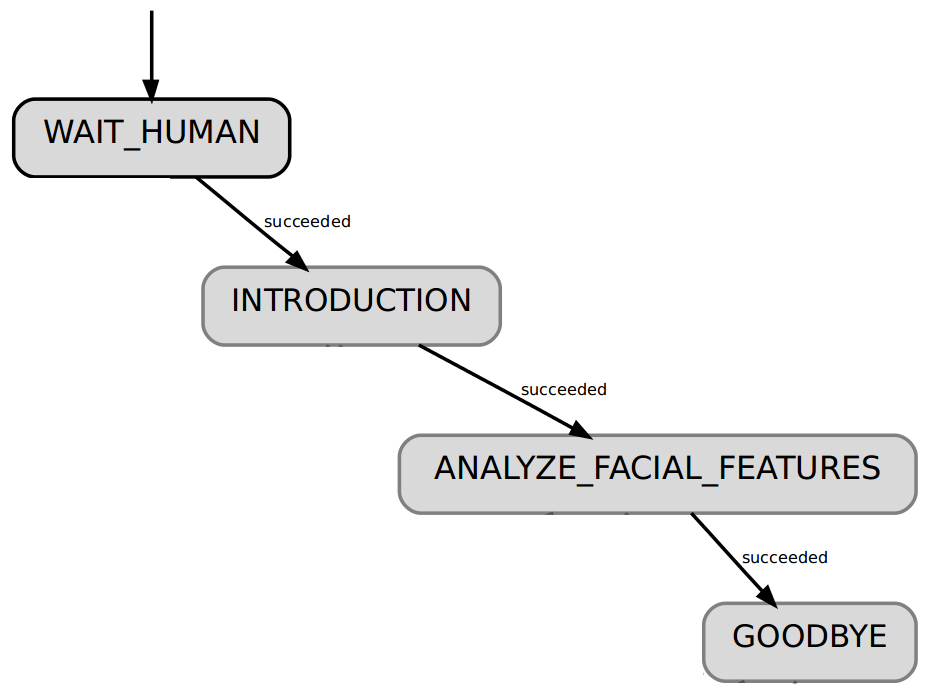
\includegraphics[width=0.7\textwidth]{human-session.png}
	\caption[SMACH: Sesión de aprendizaje de personas.]
	{\small Máquina de estado construida en SMACH para que el robot Bender adquiera datos episódicos sobre humanos. En cada sesión de aprendizaje el robot espera la presencia de un humano, para luego consultar su nombre y analizar sus características faciales. Finalmente, el robot resume los datos recopilados y se despide.}
	\label{img:human-sesssion}
\end{figure}

Finalmente, se implementó una máquina de estado que permite acceder a los datos almacenados en las sesiones de aprendizaje. En este caso, el robot es sometido a distintas preguntas episódicas sobre los datos almacenados. Por ejemplo, respondiendo consultas como: ``¿qué sucedió en el intervalo temporal T1 - T2?'', ``¿qué lugares conoce el robot?'', ``describir al humano H'' o ``describir al humano H, con el conocimiento del instante de tiempo T'', entre otras consultas.

